\documentclass{procreport}

\usepackage[dvipdfm]{graphicx}
\usepackage{ascmac}
\usepackage{moreverb}

\title{プログラミングC第1回レポート課題}
\author{小山 亮}
\date{\today}
\担当教員{樽谷 優弥, まつ本 真佑}
\所属{計算機科学コース}
\学年{2年}
\学籍番号{09B15028}
\email{u745409b@ecs.osaka-u.ac.jp}

\begin{document}
\maketitle

\section{課題1}
\subsection{課題内容}
sh-scriptをダウンロードし、sampleと名前を変え、実行パスのあるディレクトリに移動させよ。sampleに実行権限を与え実行せよ。その結果生じたhtmlファイルresult.htmlを確認せよ。
\subsection{1)、2)の作業が持つ意味}
\begin{itemize}
\item[1)]実行パスを通すとファイルを実行する際、そのファイルの入っているディレクトリを指定しなくても実行することができる。
\item[2)]sampleを実行し、ハッシュテーブルを再構築する。
\end{itemize}
\subsection{このシェルスクリプトのコマンドとしての動作説明}
簡単なhtmlファイルを出力する。
\subsection{各行の動作内容の説明}
各行にコメントを付けて下に示す。

\begin{verbatimtab}
#!/bin/sh

result=result.html	#resultをresult.htmlとする

tmpfile1=/tmp/sample.$$1
tmpfile2=/tmp/sample.$$2

if [ $# -eq 0 ]; then
	echo "Usage: $0 file [files ...]"	#""内を出力
	exit 1	#1としてシェルを閉じる
fi

trap "rm -f ${tmpfile1} ${tmpfile2}" 0 1 2 13 15	#信号を受け取るとシェルを閉じる

rm -f ${tmpfile1}	#確認なしに消去
for i in $@; do
	if [ -f ${i} ]; then
		echo ${i} >> ${tmpfile1}	#追加で書き込み
	else
		echo "can't find ${i}"	#""内を出力
	fi
done
test -f ${tmpfile1} || exit 0	#状況を1か0で返す
files="`sort < ${tmpfile1}`"

cat - > ${tmpfile2} <<EOF	#ヒアドキュメント
<html>
<head>
<title>File Contents</title>
</head>
<body>
<h1>File Contents</h1>
EOF

c=1
for i in ${files}; do
	echo "<a href=\"#${i}\">${c} ${i}</a><br>" >> ${tmpfile2}	#追加書き込み
	c=`expr ${c} + 1`
done

c=1
for i in ${files}; do
	echo "<h2><a name=\"${i}\">${c} ${i}</a></h2>" >> ${tmpfile2}	#追加書き込み
	echo '<pre>' >> ${tmpfile2}	#追加書き込み
	cat ${i} >> ${tmpfile2}	#追加書き込み
	echo '</pre>' >> ${tmpfile2}	#追加書き込み
	c=`expr ${c} + 1`
done

cat - >> ${tmpfile2}<<EOF	#ヒアドキュメント
</body>
</html>
EOF

cp ${tmpfile2} ${result}	#コピー
rm -f ${tmpfile2}	#確認なしに消去

exit 0

\end{verbatimtab}

\section{課題2}
対戦結果が書かれてあるファイルを元に、対戦結果表を出力するLaTeXファイルを出力するプログラムをperlにて作成した。作成したプログラムは\ref{sec:prog1}章に示しているものである。
\subsection{課題内容}
FIFAワールドカップ2014の1次リーグにおけるグループごとの対戦結果を記述したファイルがあり、各ファイルはプレーンテキストであり、対戦結果が表形式で記述してある。勝敗を表す記号は以下に示す。
\begin{itemize}
\item W:勝ち(win)
\item L:負け(lose)
\item D:引き分け(draw)
\end{itemize}
また、勝敗を表す記号のあとにはそれぞれその試合の各チームの特典が記述してある。これらのファイルを用いて対戦結果表のpdfファイルを出力するLaTeXファイルを生成するPerlスクリプトを作成せよ。作成するスクリプトは以下の仕様を満たすこと。

\begin{enumerate}
\item スクリプトの引数は、グループを表すA~Hまでのアルファベットとする。
\item 引数は0個以上、8個まで指定でき、指定された順序で各グループに対する対戦結果表を出力する1つのLaTeXファイルを生成する。
\item 引数が省略された場合は。すべてのグループの対戦結果表をA~Hの順に出力する1つのLaTeXファイルを生成する。
\item 不正な引数が指定された場合は、エラーメッセージを出力して終了する。
\item 生成されるLaTeXファイルの名前は、``group-指定したアルファベット全て''とする。ただし、「グループ名」は出力したグループを表すアルファベットの列とし、その順序は対戦結果表の出力順序と同一とする。 
\end{enumerate}

また、対戦結果表のpdfファイルは、以下の形式を満たすこと。

\begin{enumerate}
\item 対戦結果表はA4用紙1ページにつき1つ出力する。
\item 表はセンタリングする。
\item 対戦結果表の上にはグループ名を含むタイトルを表示する。
\item 対戦結果表は5行7列の罫線付きの表で出力する。
\item 同一国の対戦結果を表す欄は空欄とする。
\item 対戦結果には勝敗を表す記号○(勝ち)、×(負け)、△(引き分け)、点数を2行分を用いて出力する。(1行目に勝敗、2行目に点数)
\item 表の第6列、第7列、第8列は、それぞれ各国の勝ち試合数、引き分け試合数、負け試合数を出力する。
\item 対戦結果表の第1、6、7、 8列目は上下中央揃えとする。 
\end{enumerate}

\subsection{仕様}
\label{sec:charactor}
スクリプトに対する引数として、出力したい対戦結果表のリーグのアルファベットを受け取る。引数は8個まで指定することができ、A~Hまで一つずつ指定することができる。引数を指定しない場合は、A~Hまでのリーグの対戦結果表を出力する。引数に一つでも適切でない文字があると、エラーを出力し、プログラムを実行しない。生成されるLaTeXファイルは名前を``group-指定したアルファベット全て''とする。LaTeXファイルをコンパイルして結果出力されるpdfファイルは1ページに1つの表が出力されるようにする。表はセンタリングし、対戦結果の欄には、上に勝敗を表す記号を、下には得失点を記述する。また勝ち試合数、負け試合数、引き分け試合数、も記述する。これら3つと国名は上下中央揃いとする。勝ち試合数、負け試合数、引き分け試合数の表記は、表が横にはみ出ることを防ぐために、縦書きにして表の横幅を小さくした。

\subsection{処理概要}
課題2で作成したスクリプトは大きく2つの部分に分けられる。グループごとの対戦結果を記述したファイルからデータを読み込む部分とLaTeXファイルに表を出力させるソースを出力する部分である。

\subsubsection{入力部}
この部分では、データを読み込み最適な構造をした変数に格納する。まずスクリプトに与えられた引数を受け取る。これによって出力するデータなどが変わる。グループ名や表の行に対応する部分を変数に格納する。
\subsubsection{出力部}
出力部では\ref{sec:charactor}章で述べた仕様に基づいた表を出力するようなLaTeXファイルとして適切なテキストをLaTeXファイルに出力する。

\subsection{アルゴリズム}
スクリプトに与えられた引数を受け取り、扱いやすくするため、引数の入った配列をほかの配列に移す。後のためにその配列の中身を関数joinを用いて結合して変数に移す。まず引数の配列の一番目のアルファベットに対するグループのファイルを書き込みモードで読み込む。その後読み込んだデータを用意したLaTeX形式の適切な場所に出力する。それ以降は、引数の数に合わせて、その引数に対応したデータを読み込み、追加書き込みモードでLaTeXファイルに書き込む。最後にLaTeXファイルの終わりに``\textbackslash end\{document\}''を追加書き込みする。

\subsection{工夫点}
グループの国名の長さによっては表が横に長くなりすぎるため、日本語表記である勝ち試合数、負け試合数、引き分け試合数は縦書きにした。これによってグループFの表がページの外にはみ出るのを防いだ。またスクリプトの出力内容を書くとき、サンプルのpdfファイルを見ながら忠実に再現できるように書いたLaTeXファイルの内容をスクリプトに移してから適切な個所を変数で置き換える操作をした。これによりコーディングの時間短縮を図った。

\subsection{テスト結果}
groupAの対戦結果表を出力するLaTeXファイルを本プログラムによって作成した。そのLaTeXファイルを以下に示す。
\begin{screen}
\begin{verbatimtab}
\documentclass[a4j,titlepage]{jarticle}
\usepackage{multirow}
\usepackage{plext}
\begin{document}
\begin{table}[htb]
\begin{center}
\underline{2014 FIFA World Cup Stage1 Result
- Group A
 -}
\begin{tabular}{|c|c|c|c|c|c|c|c|}
\hline
&Brazil&Mexico&Croatia&Cameroon&\pbox<t>{勝ち試合数}&\pbox<t>{引き分け試合数}&\pbox<t>{負け試合数}\\
\hline
\multirow{2}{*}{Brazil}&&△&○&○&\multirow{2}{*}{2}&\multirow{2}{*}{1}
&\multirow{2}{*}{0}\\
&&0-0&3-1&4-1&&&\\
\hline
\multirow{2}{*}{Mexico}&△&&○&○&\multirow{2}{*}{2}&\multirow{2}{*}{1}
&\multirow{2}{*}{0}\\
&0-0&&3-1&1-0&&&\\
\hline
\multirow{2}{*}{Croatia}&×&×&&○&\multirow{2}{*}{1}&\multirow{2}{*}{0}
&\multirow{2}{*}{2}\\
&1-3&1-3&&4-0&&&\\
\hline
\multirow{2}{*}{Cameroon}&×&×&×&&\multirow{2}{*}{0}&\multirow{2}{*}{0}
&\multirow{2}{*}{3}\\
&1-4&0-1&0-4&&&&\\
\hline
\end{tabular}
\end{center}
\end{table}
\end{document}
\end{verbatimtab}
\end{screen}
これによるpdfファイルは\ref{sec:result}章に示す。

\section{課題3}
用意されたperl/tkによる簡単なエディタにある機能を追加した。完成したプログラムは\ref{sec:prog2}章に示しているものである。
\subsection{課題内容}

以下の機能を備えたエディタがある。

\begin{itemize}
\item Filename エントリ :テキストを書き出すファイルの名前を指定するエントリ
\item Save ボタン :テキストの書き出しを行なうボタン
\item Clear ボタン :それまでに入力したテキストを全て削除するボタン
\item Quit ボタン :エディタを終了するボタン
\item テキストフィールド:テキストを入力するフィールド
\end{itemize}
これに指定したファイル名からテキストを読み込むLoad機能、指定したファイル名からテキストをカーソル位置に読み込むInsert機能を追加せよ。また元からあるプログラムの各命令が何を行っているかを説明せよ。

\subsection{仕様}
このエディターはperl/tkによるものである。ファイル名を入力するテキストボックスは左上に表示される。その右に様々な機能を持つボタンが並ぶ。そしてそれらの下に大部分を占めるテキストフィールドがある。
\subsection{処理概要}
\subsubsection{Load機能}
これはプログラムの78から86行目に当たる。該当部分を下に示す。
\begin{screen}
\begin{verbatimtab}
    78	sub load_text{
    79	    open(INFILE, "<$savefilename")
    80		or warn("Can't open '$savefilename'"), return;
    81	    $textfield->delete( '1.0', 'end' );
    82	    while(<INFILE>){
    83		$textfield->insert( 'end', $_ );
    84	    }
    85	    close(INFILE);
    86	}
\end{verbatimtab}
\end{screen}

Load機能を持つサブルーチンを呼び出すボタンを作る。実態であるサブルーチンでは、まず今テキストフィールドにあるテキストを削除する。その後指定したファイルのテキストをテキストフィールドに表示する。
\subsubsection{Insert機能}
これはプログラムの88から95行目に当たる。該当部分を下に示す。
\begin{screen}
\begin{verbatimtab}
    88	sub insert_text{
    89	    open(INFILE, "<$savefilename")
    90		or warn("Can't open '$savefilename'"), return;
    91	    while(<INFILE>){
    92		$textfield->insert( 'insert', $_ );
    93	    }
    94	    close(INFILE);
    95	}
\end{verbatimtab}
\end{screen}

Insert機能を持つサブルーチンを呼び出すボタンを作る。実態であるサブルーチンでは、指定したファイルのテキストをカーソルの位置にテキストフィールドに表示する。
\subsection{アルゴリズム}
\subsubsection{Load機能}
ファイル名を指定するテキストボックスからファイル名を読み取り、そのファイルを読み取り形式で開く。開けなければエラーを返す。テキストフィールドの内容を消去する。その後、指定したファイルを行ごとに最後までテキストフィールドに挿入していく。
\subsubsection{Insert機能}
ファイル名を指定するテキストボックスからファイル名を読み取り、そのファイルを読み取り形式で開く。開けなければエラーを返す。カーソル位置から指定したファイルを行ごとに最後までテキストフィールドに挿入していく。
\subsection{工夫点}
ファイルハンドルを意味のあるものにし、わかりやすいようにした。
\subsection{テスト結果}
テストした結果期待した機能が備わっていることを確認した。しかしInsert機能を使用したときに、最後に改行がはいていた。
\subsection{スクリプトの説明}
\begin{itemize}
\item use Tk; - Tk.pmがロードされる
\item -$>$ - メソッドを呼び出す
\item MaiLoop; - メインループを呼び出す
\end{itemize}

\section{全体の感想}
c言語でもファイルを扱うプログラムを作成したが、perlで書いた方が簡単だったように感じる。またperlでは変数宣言が必要ないなど、簡単な部分もあった。しかし、簡略化されすぎるとどこかで不都合が起きやすくなってしまうのではないかとも感じた。

\newpage
\appendix

\section{対戦結果表の出力(groupA)}
\label{sec:result}

\begin{figure}[h]
\begin{center}
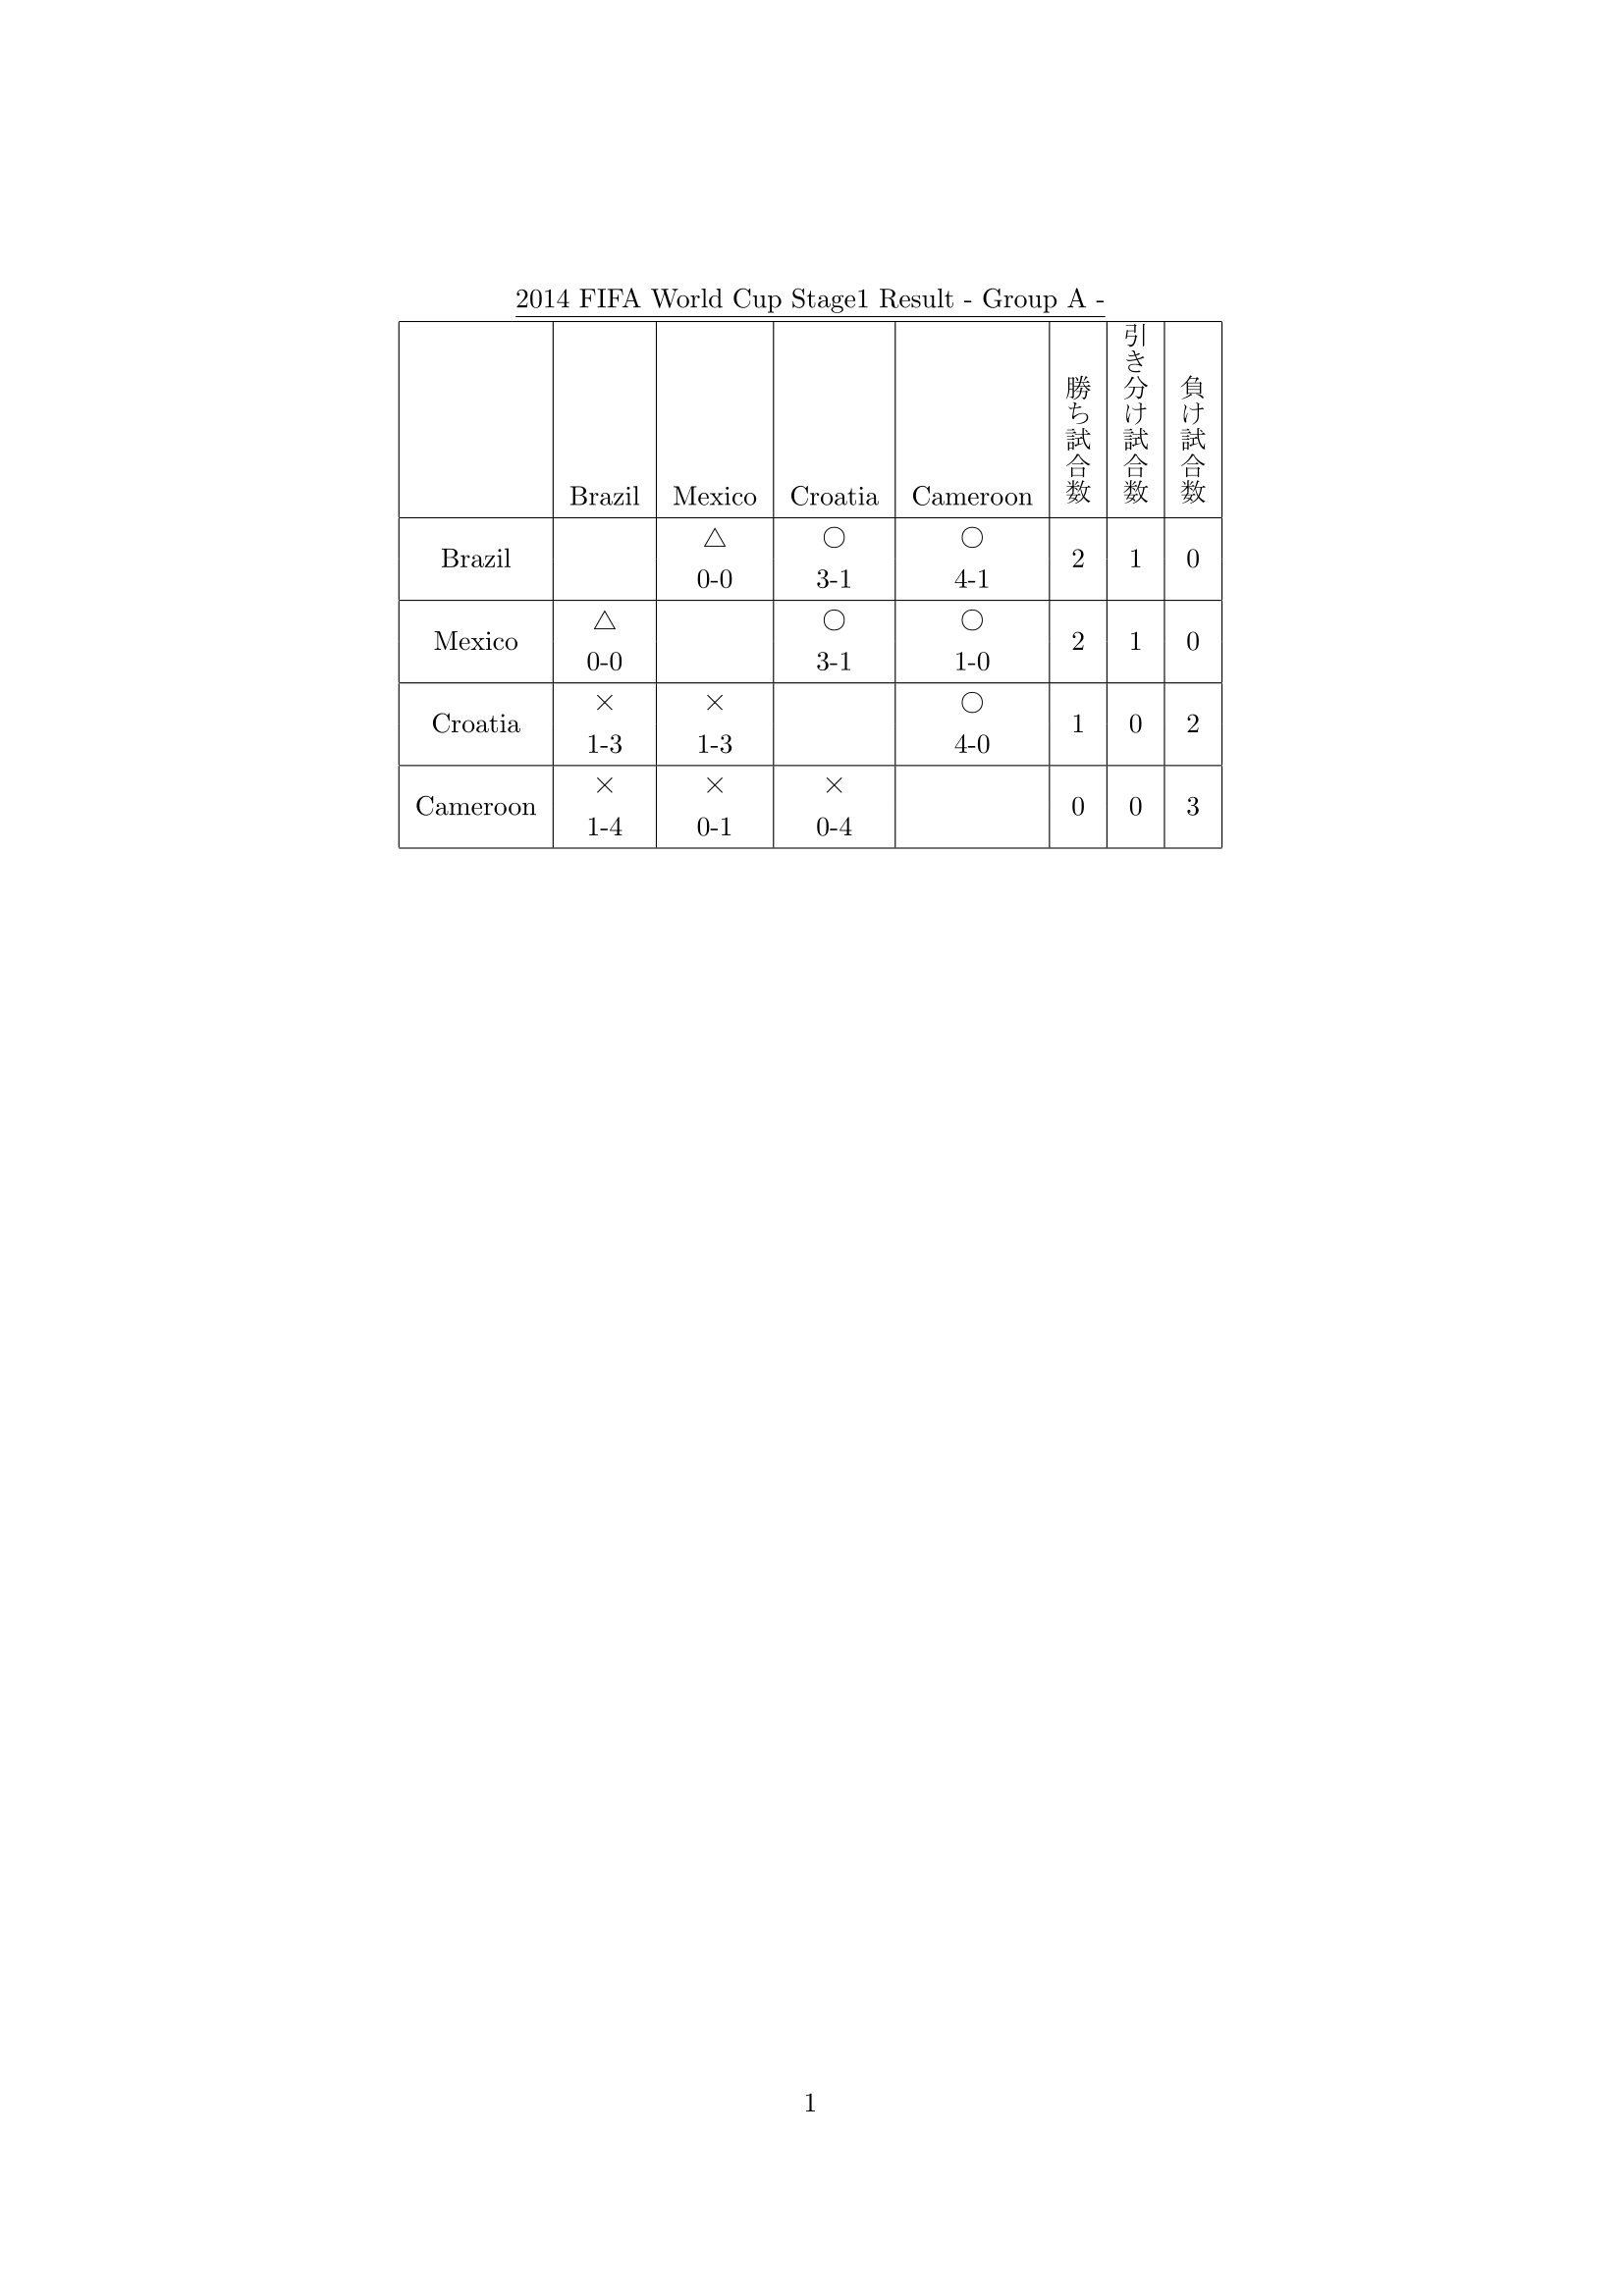
\includegraphics[width=12cm,clip]{group-A-1.png}
\end{center}
\caption{groupA}
\end{figure} 

\section{プログラムリスト}

\subsection{表を作成するLaTeXファイルを作成するプログラム}
\label{sec:prog1}
\begin{verbatimtab}
     1	#!/usr/local/bin/perl
     2	
     3	$i=0;
     4	for($m=0;$m<@ARGV;$m++){
     5		if($ARGV[$m]!="[A-H]"){
     6			print"Error(incorrect letter)\n";
     7			$i=1;
     8		}
     9	}
    10	
    11	if($i==0){
    12		if(@ARGV){
    13			@al=@ARGV;
    14		}
    15		else{
    16			@al=(A,B,C,D,E,F,G,H);
    17		}
    18	
    19		$name=join("" , @al);
    20	
    21		open(TABLE,"< group$al[0]");
    22		@line=<TABLE>;
    23		close(TABLE);
    24	
    25		chomp($line[0]);
    26		chomp($line[2]);
    27	
    28		for($i=0;$i<4;$i++){
    29			foreach(@team[$i]){
    30				$_=[split(/\s+/,$line[$i+4])];
    31			}
    32		}
    33	
    34		for($i=0;$i<4;$i++){
    35			$team[$i][0]=~ s/[_]/\\_/g;
    36		}
    37	
    38		@data=(
    39			[0,0,0],
    40			[0,0,0],
    41			[0,0,0],
    42			[0,0,0]
    43		);
    44	#nチーム目の[勝ち数,負け数,引き分け数]
    45	
    46		for($i=0;$i<4;$i++){	#各行に対して勝ち負け引き分けを表す文字を記号で当てる
    47			for($k=0;$k<8;$k++){
    48				if($team[$i][$k]=~/^W$/){
    49					$team[$i][$k]="\○";
    50					$data[$i][0]++;
    51				}
    52				elsif($team[$i][$k]=~/^L$/){
    53					$team[$i][$k]="\×";
    54					$data[$i][1]++;
    55				}
    56				elsif($team[$i][$k]=~/^D$/){
    57					$team[$i][$k]="\△";
    58					$data[$i][2]++;
    59				}
    60			}
    61		}
    62	
    63		open(TEX,"> group-$name.tex");
    64		print TEX <<"EOT";	#texファイルの内容
    65	\\documentclass[a4j,titlepage]{jarticle}
    66	\\usepackage{multirow}
    67	\\usepackage{plext}
    68	\\begin{document}
    69	\\begin{table}[htb]
    70	\\begin{center}
    71	\\underline{$line[0]- $line[2] -}
    72	\\begin{tabular}{|c|c|c|c|c|c|c|c|}
    73	\\hline
    74	&$team[0][0]&$team[1][0]&$team[2][0]&$team[3][0]&\\pbox<t>{勝ち試合数}&\\
pbox<t>{引き分け試合数}&\\pbox<t>{負け試合数}\\\\
    75	\\hline
    76	\\multirow{2}{*}{$team[0][0]}&&$team[0][2]&$team[0][4]&$team[0][6]&\\
multirow{2}{*}{$data[0][0]}&\\multirow{2}{*}{$data[0][2]}&\\multirow{2}{*}{
$data[0][1]}\\\\
    77	&&$team[0][3]&$team[0][5]&$team[0][7]&&&\\\\
    78	\\hline
    79	\\multirow{2}{*}{$team[1][0]}&$team[1][1]&&$team[1][4]&$team[1][6]&\\
multirow{2}{*}{$data[1][0]}&\\multirow{2}{*}{$data[1][2]}&\\multirow{2}{*}{
$data[1][1]}\\\\
    80	&$team[1][2]&&$team[1][5]&$team[1][7]&&&\\\\
    81	\\hline
    82	\\multirow{2}{*}{$team[2][0]}&$team[2][1]&$team[2][3]&&$team[2][6]&\\
multirow{2}{*}{$data[2][0]}&\\multirow{2}{*}{$data[2][2]}&\\multirow{2}{*}{
$data[2][1]}\\\\
    83	&$team[2][2]&$team[2][4]&&$team[2][7]&&&\\\\
    84	\\hline
    85	\\multirow{2}{*}{$team[3][0]}&$team[3][1]&$team[3][3]&$team[3][5]&&\\
multirow{2}{*}{$data[3][0]}&\\multirow{2}{*}{$data[3][2]}&\\multirow{2}{*}{
$data[3][1]}\\\\
    86	&$team[3][2]&$team[3][4]&$team[3][6]&&&&\\\\
    87	\\hline
    88	\\end{tabular}
    89	\\end{center}
    90	\\end{table}
    91	EOT
    92		close(TEX);
    93	
    94		for($m=1;$m<@al;$m++){
    95			open(TABLE,"< group$al[$m]");
    96			@line=<TABLE>;
    97			close(TABLE);
    98	
    99			chomp($line[0]);
   100			chomp($line[2]);
   101	
   102			for($i=0;$i<4;$i++){
   103				foreach(@team[$i]){
   104					$_=[split(/\s+/,$line[$i+4])];
   105				}
   106			}
   107	
   108			for($i=0;$i<4;$i++){
   109				$team[$i][0]=~ s/[_]/\\_/g;
   110			}
   111	
   112			@data=(
   113				[0,0,0],
   114				[0,0,0],
   115				[0,0,0],
   116				[0,0,0]
   117			);
   118	#nチーム目の[勝ち数,負け数,引き分け数]
   119	
   120			for($i=0;$i<4;$i++){
   121				for($k=0;$k<8;$k++){
   122					if($team[$i][$k]=~/^W$/){
   123						$team[$i][$k]="\○";
   124						$data[$i][0]++;
   125					}
   126					elsif($team[$i][$k]=~/^L$/){
   127						$team[$i][$k]="\×";
   128						$data[$i][1]++;
   129					}
   130					elsif($team[$i][$k]=~/^D$/){
   131						$team[$i][$k]="\△";
   132						$data[$i][2]++;
   133					}
   134				}
   135			}
   136	
   137			open(TEX,">> group-$name.tex");
   138			print TEX <<"EOT";
   139	\\newpage
   140	\\begin{table}[htb]
   141	\\begin{center}
   142	\\underline{$line[0]- $line[2] -}
   143	\\begin{tabular}{|c|c|c|c|c|c|c|c|}
   144	\\hline
   145	&$team[0][0]&$team[1][0]&$team[2][0]&$team[3][0]&\\pbox<t>{勝ち試合数}&\\
pbox<t>{引き分け試合数}&\\pbox<t>{負け試合数}\\\\
   146	\\hline
   147	\\multirow{2}{*}{$team[0][0]}&&$team[0][2]&$team[0][4]&$team[0][6]&\\
multirow{2}{*}{$data[0][0]}&\\multirow{2}{*}{$data[0][2]}&\\multirow{2}{*}{
$data[0][1]}\\\\
   148	&&$team[0][3]&$team[0][5]&$team[0][7]&&&\\\\
   149	\\hline
   150	\\multirow{2}{*}{$team[1][0]}&$team[1][1]&&$team[1][4]&$team[1][6]&\\
multirow{2}{*}{$data[1][0]}&\\multirow{2}{*}{$data[1][2]}&\\multirow{2}{*}{
$data[1][1]}\\\\
   151	&$team[1][2]&&$team[1][5]&$team[1][7]&&&\\\\
   152	\\hline
   153	\\multirow{2}{*}{$team[2][0]}&$team[2][1]&$team[2][3]&&$team[2][6]&\\
multirow{2}{*}{$data[2][0]}&\\multirow{2}{*}{$data[2][2]}&\\multirow{2}{*}{
$data[2][1]}\\\\
   154	&$team[2][2]&$team[2][4]&&$team[2][7]&&&\\\\
   155	\\hline
   156	\\multirow{2}{*}{$team[3][0]}&$team[3][1]&$team[3][3]&$team[3][5]&&\\
multirow{2}{*}{$data[3][0]}&\\multirow{2}{*}{$data[3][2]}&\\multirow{2}{*}{
$data[3][1]}\\\\
   157	&$team[3][2]&$team[3][4]&$team[3][6]&&&&\\\\
   158	\\hline
   159	\\end{tabular}
   160	\\end{center}
   161	\\end{table}
   162	EOT
   163			close(TEX);
   164		}
   165	
   166		open(TEX,">> group-$name.tex");
   167		print TEX "\\end{document}";
   168		close(TEX);
   169	}
\end{verbatimtab}

\subsection{簡単なエディターのプログラム}
\label{sec:prog2}
\begin{verbatimtab}

     1	#!/usr/local/bin/perl
     2	#
     3	# Very Simple Editor
     4	#
     5	
     6	use Tk;
     7	
     8	$mw = MainWindow->new();
     9	$mw->title("Very Simple Editor");
    10	
    11	#
    12	# ボタンとファイル名エントリを格納するフレームを作成
    13	#
    14	$top = $mw->Frame(-borderwidth => 10);
    15	$top->pack(-side => 'top', -fill => 'x');
    16	
    17	#
    18	# ボタンとファイル名エントリを作成, 配置
    19	#
    20	$quit = $top->Button(-text => 'Quit', -command => sub { exit });
    21	$clear = $top->Button(-text => 'Clear', -command => \&clear_text);
    22	$save = $top->Button(-text => 'Save', -command => \&save_text);
    23	$load = $top->Button(-text => 'Load', -command => \&load_text);
    24	$insert = $top->Button(-text => 'Insert', -command => \&insert_text);
    25	$label = $top->Label(-text => 'Filename:', -padx => 0);
    26	$filename = $top->Entry(-width => 20,
    27				-relief => 'sunken',
    28				-textvariable => \$savefilename);
    29	$label->pack(-side => 'left');
    30	$filename->pack(-side => 'left');
    31	$quit->pack(-side => 'right');
    32	$clear->pack(-side => 'right');
    33	$save->pack(-side => 'right');
    34	$load->pack(-side => 'right');
    35	$insert->pack(-side => 'right');
    36	
    37	#
    38	# エディットに利用するテキストウィジェットを作成
    39	#
    40	$textframe = $mw->Frame();
    41	$scroll = $textframe->Scrollbar();
    42	$textfield = $textframe->Text(-width => 80,
    43				      -height => 25,
    44				      -borderwidth => 2,
    45				      -relief => 'sunken',
    46				      -setgrid => 1,
    47				      -yscrollcommand => ['set' => $scroll]);
    48	$scroll->configure(-command => ['yview' => $textfield]);
    49	$scroll->pack(-side => 'right', -fill => 'y');
    50	$textfield->pack(-side => 'left', -fill => 'both', -expand => 1);
    51	$textframe->pack(-side => 'top', -fill => 'both', -expand => 1);
    52	
    53	#
    54	# 表示
    55	#
    56	MainLoop;
    57	
    58	#
    59	# Clearボタンに対応する手続き
    60	# エディット中のテキストをすべて削除する
    61	#
    62	sub clear_text {
    63	    $textfield->delete('1.0','end');
    64	}
    65	
    66	#
    67	# Saveボタンに対応する手続き
    68	# filenameエントリに記述されたファイル名でファイルをオープンし, 
    69	# テキストウィジェットの内容をそのファイルへ書き込む
    70	#
    71	sub save_text {
    72	    open(OUTFILE, ">$savefilename")
    73		or warn("Can't open '$savefilename'"), return;
    74	    print OUTFILE $textfield->get('1.0','end');
    75	    close(OUTFILE);
    76	}
    77	
    78	sub load_text{
    79	    open(INFILE, "<$savefilename")
    80		or warn("Can't open '$savefilename'"), return;
    81	    $textfield->delete( '1.0', 'end' );
    82	    while(<INFILE>){
    83		$textfield->insert( 'end', $_ );
    84	    }
    85	    close(INFILE);
    86	}
    87	
    88	sub insert_text{
    89	    open(INFILE, "<$savefilename")
    90		or warn("Can't open '$savefilename'"), return;
    91	    while(<INFILE>){
    92		$textfield->insert( 'insert', $_ );
    93	    }
    94	    close(INFILE);
    95	}

\end{verbatimtab}

\end{document}